\chapter{Graphs}
Here, I will simply show you how to import graphs in .svg format, add captions to them, and resize them properly.

\begin{figure}[!ht]
  \centering
  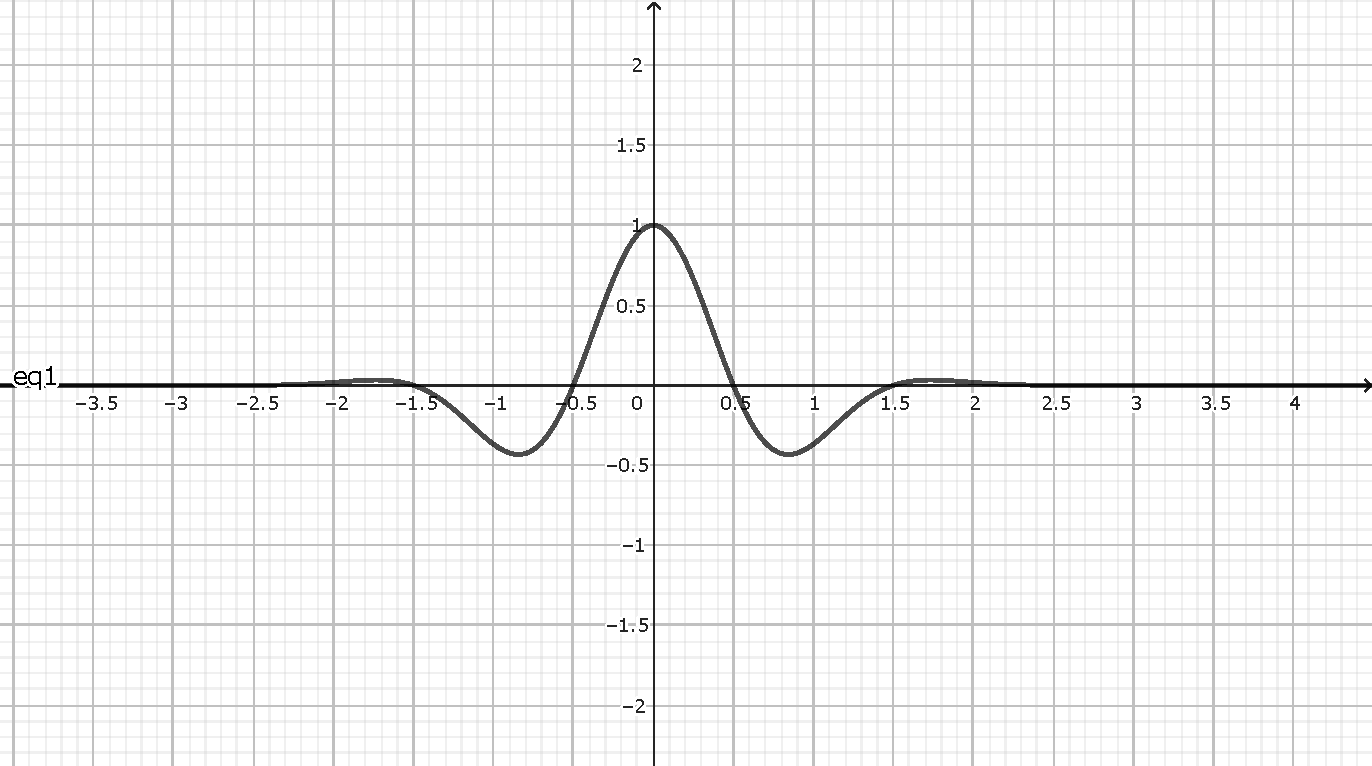
\includegraphics[width=0.8\textwidth]{svg-inkscape/esempio_geogebra_svg-raw.pdf}
  \caption{Example of including a PDF document.}
  \label{fig:pdf-example}
\end{figure}


\begin{figure}[!ht]
	\centering
	% Import the SVG image, applying cropping and resizing
	\includesvg[width=0.8\textwidth,inkscapelatex=false]{res/svg/esempio_geogebra}
	\caption{This is the example graph I created with Geogebra, with a caption and an associated label. To import SVG graphs, you need to install Inkscape, add it to the system path (watch out for the path, nothing works if you don’t do this, it’s usually \texttt{C:/Program Files/Inkscape/bin}), and modify the compiler flag by adding \texttt{-shell-escape}. If you are on Overleaf, it does this automatically (lucky you who didn’t waste 1 hour figuring this out, as a revenge, I write the most important things in the captions xD).}
	\label{graph:esempiografico}
\end{figure}

\hfill

\begin{figure}[!ht]
	\centering
	% Import the SVG image, applying cropping and resizing
	\includesvg[width=0.8\textwidth,inkscapelatex=false]{res/svg/2d_example}
	\caption{This is the 2d graph I created with matplotlib, see script.}
	\label{graph:esempiograficopy}
\end{figure}

\hfill

\begin{figure}[!ht]
	\centering
	% Import the SVG image, applying cropping and resizing
	\includesvg[width=0.8\textwidth,inkscapelatex=false]{res/svg/3d_continuous_example}
	\caption{This is the continuous 3d graph I created with matplotlib, see script.}
	\label{graph:esempiograficopy2}
\end{figure}

\hfill

\begin{figure}[!ht]
	\centering
	% Import the SVG image, applying cropping and resizing
	\includesvg[width=0.8\linewidth,inkscapelatex=false]{res/svg/3d_wireframe_example}
	\caption{This is the continuous 3d graph I created with matplotlib, see script.}
	\label{graph:esempiograficopy3}
\end{figure}

\hfill

\begin{figure}[!ht]
	\centering
	% Import the SVG image, applying cropping and resizing
	\includesvg[width=0.8\linewidth,inkscapelatex=false]{res/svg/esempioMappaConcettuale.drawio}
	\caption{A dummy conceptual map created with the draw.io online editor.}
	\label{graph:esempioMappaConcettuale}
\end{figure}

\hfill

\begin{figure}[!ht]
	\centering
	% Import the SVG image, applying cropping and resizing
	\includesvg[width=0.8\linewidth,inkscapelatex=false]{res/svg/esempioCircuito.drawio}
	\caption{A basic circuit created with the draw.io online editor.}
	\label{graph:esempioCircuito}
\end{figure}

\hfill

If you open the .tex file, you will notice that I have inserted the \texttt{\textbackslash href} command between each graph. This is to prevent \LaTeX from optimizing the space by fragmenting the bulleted list below between the graphs. Don’t believe me? Try it and see what chaos it creates.

Labels can be associated with many objects in Matlab, make good use of them! Especially when you need to refer to formulas, tables, or graphs in your text. Here are all the ways you can reference an object with an associated label:
\begin{enumerate}
	\item \texttt{\textbackslash ref\{graph:esempiografico\}}: To refer to the number associated with the label, such as a figure, table, section, etc. (example: Figure~\ref{graph:esempiografico}).
	\item \texttt{\textbackslash pageref\{graph:esempiografico\}}: To refer to the page number where the labeled object appears (example: See page~\pageref{graph:esempiografico}).
	\item \texttt{\textbackslash hyperref\{graph:esempiografico\}}: If you use the \texttt{hyperref} package, you can click the reference to go directly to the figure, table, etc.
	\item \texttt{\textbackslash eqref\{graph:esempiografico\}}: To refer to an equation, if the label has been applied to an equation environment (example: as shown in equation~\eqref{graph:esempiografico}).
\end{enumerate}
